\chapter{Estructura de la ecuación de cotización}
\label{cap:estructura}

Este es el capítulo central del trabajo. Se establece aquí la estructura analítica
exacta de la función de valoración $\VP$ definida en \cref{eq:canonica}, y se
muestra que difiere en tres aspectos sustanciales de la que la práctica actuarial
supone. De esa estructura se derivan, en el \cref{cap:metodos}, las propiedades de
convergencia de los métodos iterativos.

A lo largo del capítulo se trabaja con la forma canónica
\begin{equation}
\label{eq:canonica-rep}
  \VP(M)\;=\;\underbrace{\sum_{t=1}^{N} w_t\,\max\{a_tM,\,b_t\}}_{\textstyle \VP_{\mathrm{ren}}(M)}
            \;+\;\underbrace{\sum_{t=1}^{N} c_t\,\med\bigl(5b_t,\;a_tM,\;10b_t\bigr)}_{\textstyle \VP_{\mathrm{auf}}(M)},
\end{equation}
con $w_t,c_t\ge0$ y $a_t,b_t>0$ independientes de $M$
(\cref{prop:forma-canonica}). Se supone en todo el capítulo que $w_1>0$, de modo que el primer periodo con $a_1=1$ y $b_1=S_0$ aporta positivamente a la renta.

\section{Regularidad básica}

\begin{proposition}[Continuidad y Lipschitz]
\label{prop:lipschitz}
$\VP$ es continua en $[0,\infty)$ y globalmente Lipschitz con constante
\[
  L \;=\; \sum_{t=1}^{N}\bigl(w_t+c_t\bigr)a_t \;<\;\infty .
\]
\end{proposition}
\begin{proof}
Cada $u\mapsto\max\{a_tu,b_t\}$ es $a_t$-Lipschitz y cada
$u\mapsto\med(5b_t,a_tu,10b_t)$ es también $a_t$-Lipschitz por el
\cref{lem:recorte}. La suma finita de funciones Lipschitz con pesos no negativos
$w_t,c_t$ es Lipschitz con constante la suma ponderada. La finitud de $L$ se sigue
de que $N=\datoNMeses$ es finito.
\end{proof}

Obsérvese que la finitud de $L$ no requiere ninguna hipótesis de convergencia de
series: es consecuencia directa del horizonte acotado
$\nu_t=0$ para $t\ge\datoVigenciaCorte$ de \cref{eq:vigencia}. Este es un punto
donde el modelo discreto real es \emph{más simple} que su idealización continua, y
donde el borrador original de este trabajo introducía hipótesis innecesarias\footnote{El borrador enunciaba un lema de convergencia absoluta de la serie que define el valor presente, con hipótesis de sumabilidad sobre los factores de descuento. Sobre una suma finita esas hipótesis son vacuas. Se conservan aquí, en cambio, las consecuencias: continuidad y carácter Lipschitz, que sí se usan.}.

\begin{proposition}[Linealidad a trozos]
\label{prop:pl}
$\VP$ es lineal a trozos en $[0,\infty)$, con a lo sumo
$3(\datoNAniosMax+1)=\datoNQuiebresMax$ puntos de quiebre.
\end{proposition}
\begin{proof}
Por el \cref{lem:pl-cerrado} la clase de funciones lineales a trozos es cerrada
bajo sumas finitas, $\max$ y $\min$; \cref{eq:canonica-rep} es una suma finita de
tales operaciones sobre funciones afines. La cota sobre el número de quiebres se
demuestra en el \cref{thm:quiebres}.
\end{proof}

\section{La región plana}

El primer resultado corrige el enunciado clásico de monotonía estricta.

\begin{theorem}[Región plana]
\label{thm:region-plana}
Sea $S_0$ el salario mínimo vigente. Entonces
\[
  \VP(M)\;=\;\VP(0)\;=\;\sum_{t=1}^N w_tb_t+5\sum_{t=1}^N c_tb_t
  \qquad\text{para todo } M\in[0,S_0].
\]
En particular $\VP$ \textbf{no} es estrictamente creciente en $[0,\infty)$, y
$\VP'\equiv0$ en el interior de $[0,S_0]$.
\end{theorem}
\begin{proof}
Sea $M\in[0,S_0]$ y $t\in\{1,\dots,N\}$ arbitrario. Como $\delta\ge0$, de
\cref{eq:factor-ipc} se sigue $\phi_{n}\ge\tau_{n}$ para todo $n\ge0$, y por tanto
$b_t=S_0\phi_t\ge S_0\tau_t\ge M\tau_t=a_tM$. Luego
\[
  \max\{a_tM,\,b_t\}=b_t ,
\]
independientemente de $M$. Para el término del auxilio funerario, de
$a_tM\le b_t<5b_t$ se obtiene
\[
  \med\bigl(5b_t,\,a_tM,\,10b_t\bigr)=5b_t ,
\]
también independiente de $M$. Sustituyendo ambos en \cref{eq:canonica-rep} se
obtiene la expresión del enunciado, constante en $M$.
\end{proof}

\begin{remark}[Lectura actuarial]
El resultado no es un artificio matemático: dice algo económicamente evidente una
vez enunciado. Si el capital solo alcanza para una mesada por debajo del salario
mínimo, la garantía legal obliga a pagar el salario mínimo de todos modos, de modo
que \emph{el costo del contrato deja de depender de la mesada nominal
contratada\footnote{Dicho de otro modo: por debajo del salario mínimo, la mesada contratada es una ficción contable. Lo que la aseguradora se obliga a pagar es el salario mínimo, y eso es lo que cuesta. La consecuencia matemática --- pérdida de inyectividad --- es el reflejo exacto de una consecuencia económica evidente una vez enunciada.}}. La función de valoración se satura, y con ella se pierde la
información necesaria para invertirla.
\end{remark}

\begin{corollary}[Condición de capital mínimo]
\label{cor:capital-minimo}
Sea $\KA_{\min}=\VP(S_0)$. En el dominio admisible $[S_0,\infty)$,
el problema tiene ninguna solución si $\KA<\KA_{\min}$,
la solución única $M=S_0$ si $\KA=\KA_{\min}$ y una solución única
$M>S_0$ si $\KA>\KA_{\min}$. En la extensión a $[0,\infty)$,
el caso de igualdad tiene como conjunto de soluciones $[0,S_0]$.
\end{corollary}
\begin{proof}
La región plana y la monotonía implican $\VP(M)\ge\KA_{\min}$.
La monotonía estricta en $[S_0,\infty)$ da la unicidad en la igualdad.
La existencia y unicidad por encima del mínimo se obtienen en el
\cref{thm:existencia} por continuidad y crecimiento no acotado.
\end{proof}

Para la póliza de referencia de este trabajo,
$\KA_{\min}=\datoKAmin$ pesos, es decir aproximadamente
$\datoKAminMill$ millones. La \cref{fig:region-plana} ilustra los tres casos.

\begin{figure}[H]
\centering
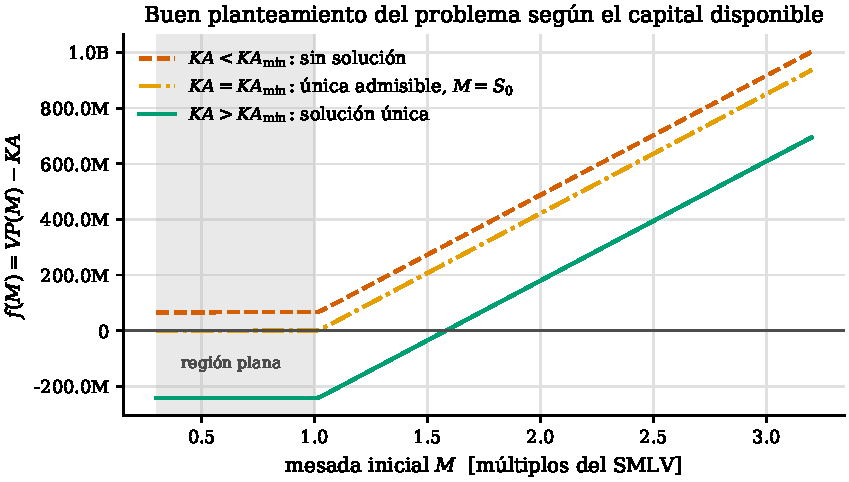
\includegraphics[width=.86\textwidth]{figuras/fig_region_plana}
\caption[Buen planteamiento del problema de cotización]{Los tres regímenes del
\cref{cor:capital-minimo}. Si el capital es insuficiente, $f$ no corta el eje y no
existe mesada admisible; si es exactamente el mínimo, $f$ se anula en todo el
intervalo $[0,\SMLV]$ de la extensión matemática. En el dominio admisible, la igualdad tiene la solución única $M=S_0$.}
\label{fig:region-plana}
\end{figure}

\begin{criticism}[Diagnóstico de insuficiencia y fallo numérico]
\label{crit:no-convergencia}
La implementación busca la raíz en $[S_0,25S_0]$. La insuficiencia
de capital debe diagnosticarse comparando $\KA$ con $\VP(S_0)$,
como establece el \cref{cor:capital-minimo}. El fracaso de un método
no basta para ese diagnóstico: también puede deberse a estancamiento
o a una raíz por encima del extremo superior. Devolver el salario mínimo
en tales situaciones no certifica la igualdad actuarial ni identifica
la financiación del importe pagado. La recomendación R1 exige separar
la inexistencia de una mesada financiable de los estados numéricos de
la búsqueda.
\end{criticism}

\section{Monotonía}

\begin{proposition}[Monotonía]
\label{prop:monotonia}
$\VP$ es no decreciente en $[0,\infty)$, y estrictamente creciente en
$[S_0,\infty)$.
\end{proposition}
\begin{proof}
La monotonía no estricta es inmediata: cada sumando de \cref{eq:canonica-rep} es no
decreciente en $M$ ($\max$ y $\med$ de funciones no decrecientes) y los pesos son
no negativos.

Para la monotonía estricta en $[S_0,\infty)$, sean $S_0\le M_1<M_2$. Considérese
el primer periodo, $t=1$, para el cual $n(1)=0$ y por tanto $a_1=\tau_1=1$,
$b_1=S_0\phi_1=S_0$. Entonces $a_1M_2=M_2>S_0=b_1$, luego
\[
  \max\{a_1M_2,b_1\}=M_2 \;>\; \max\{a_1M_1,b_1\}=\max\{M_1,S_0\}=M_1 ,
\]
donde la última igualdad usa $M_1\ge S_0$. Como $w_1>0$ por hipótesis y todos los
demás sumandos son no decrecientes, se concluye $\VP(M_1)<\VP(M_2)$.
\end{proof}

\begin{remark}
La prueba de monotonía estricta utiliza un término con peso positivo
del año calendario de valoración. En la derivada derecha en $S_0$
contribuyen todos los periodos con $n(t)=0$, no únicamente el primero.
Los periodos posteriores al primer reajuste tienen sus quiebres a la
derecha si $\delta>0$. La pendiente inmediatamente superior a $S_0$
es menor que la del tramo comercial, lo que hace más exigentes los
casos con capital cercano al mínimo.

\end{remark}

\section{El conjunto de puntos de quiebre}

\begin{theorem}[Caracterización de los quiebres]
\label{thm:quiebres}
Defínase, para $n=0,1,\dots,n_{\max}$ con
$n_{\max}=\lfloor(\datoVigenciaCorte-1)/12\rfloor=\datoNAniosMax$,
\[
  \rho_n \;=\; \frac{\phi_n}{\tau_n}\;=\;
  \begin{cases}
    1, & n=0,\\[2pt]
    \dfrac{1+\pi_1+\delta}{1+\pi_1}, & n=1,\\[4pt]
    \dfrac{(1+\pi_1+\delta)(1+\pi_2+\delta)}{(1+\pi_1)(1+\pi_2)}\,\rho^{\,n-2},
      & n\ge2,
  \end{cases}
  \qquad
  \rho\;=\;\frac{1+\pi_\infty+\delta}{1+\pi_\infty}.
\]
Entonces el conjunto de puntos de no diferenciabilidad de $\VP$ está contenido en
\begin{equation}
\label{eq:quiebres}
  \mathcal{B}\;=\;\underbrace{\bigl\{S_0\rho_n\bigr\}_{n=0}^{n_{\max}}}_{\text{racimo I}}
   \;\cup\;\underbrace{\bigl\{5S_0\rho_n\bigr\}_{n=0}^{n_{\max}}}_{\text{racimo II}}
   \;\cup\;\underbrace{\bigl\{10S_0\rho_n\bigr\}_{n=0}^{n_{\max}}}_{\text{racimo III}} .
\end{equation}
La sucesión $\{\rho_n\}$ es estrictamente creciente si $\delta>0$, con
$\rho_0=1$. Para la parametrización considerada,
$\rho_{n_{\max}}\approx\datoAnchoRacimo<2$; los tres racimos quedan
contenidos en los siguientes intervalos disjuntos:
\[
  \mathcal{B}\subset
  [S_0,\;\rho_{n_{\max}}S_0]\;\cup\;
  [5S_0,\;5\rho_{n_{\max}}S_0]\;\cup\;
  [10S_0,\;10\rho_{n_{\max}}S_0].
\]
\end{theorem}
\begin{proof}
Por el \cref{lem:pl-cerrado}, el conjunto de quiebres de la suma
\cref{eq:canonica-rep} está contenido en la unión de los conjuntos de quiebres de
sus sumandos. El sumando $t$-ésimo del primer bloque,
$M\mapsto\max\{a_tM,b_t\}$, tiene un único quiebre en $M=b_t/a_t$. El del segundo
bloque, $M\mapsto\med(5b_t,a_tM,10b_t)$, tiene dos, en $M=5b_t/a_t$ y
$M=10b_t/a_t$.

Ahora bien, $b_t/a_t = S_0\phi_t/\tau_t = S_0\rho_{n(t)}$ depende de $t$
\emph{únicamente a través del año calendario} $n(t)$, porque los factores de
indexación de \cref{eq:factor-ipc} se actualizan una vez al año.\footnote{Es el punto técnico decisivo de la demostración. Si la indexación fuese continua --- si la mesada creciera mes a mes en lugar de dar un salto anual --- habría un quiebre distinto por cada uno de los $\datoNMeses$ periodos, y el conjunto candidato seguiría siendo finito, aunque podría tener más elementos. La estructura discreta del reajuste es lo que hace tratable el problema.} Como
$\nu_t=0$ para $t\ge\datoVigenciaCorte$, los índices $t$ con peso no nulo
satisfacen $n(t)\le n_{\max}$. Esto da \cref{eq:quiebres}.

La monotonía estricta de $\rho_n$ para $\delta>0$ se sigue de que cada factor
$(1+\pi+\delta)/(1+\pi)>1$. Finalmente, los racimos son disjuntos porque
$\rho_{n_{\max}}<2$, luego
$\rho_{n_{\max}}S_0<5S_0$ y $5\rho_{n_{\max}}S_0<10S_0$.
\end{proof}

\begin{corollary}[Región afín]
\label{cor:region-afin}
$\VP$ es \textbf{afín} en cada uno de los intervalos
\[
  \bigl[\rho_{n_{\max}}S_0,\;5S_0\bigr],\qquad
  \bigl[5\rho_{n_{\max}}S_0,\;10S_0\bigr],\qquad
  \bigl[10\rho_{n_{\max}}S_0,\;\infty\bigr).
\]
\end{corollary}

El \cref{cor:region-afin} es el resultado con mayor consecuencia práctica de todo
el trabajo. El primero de esos intervalos, aproximadamente
$[1{,}15\,S_0,\;5\,S_0]$, contiene las mesadas de la muestra examinada: en los dos conjuntos reales del \cref{cap:resultados}
(\datoNReales{} cotizaciones de renta vitalicia y \datoNRealesRP{} registros
adicionales), todas las mesadas resultantes caen entre
$\datoMultMin$ y $\datoMultMax$ salarios mínimos, con media $\datoMultMedia$. Es
decir: \emph{el intervalo que contiene las mesadas de esta muestra es un tramo
afín}, y Newton con su pendiente exacta termina en un paso cuando el arranque también está en el interior de ese tramo. Así
ocurre (\cref{thm:terminacion-finita} y \cref{tab:terminacion}).

\begin{remark}[Por qué los racimos son tan estrechos]
La razón geométrica es $\rho=\datoRhoQuiebre$, esto es, un
$\datoRhoQuiebrePct\%$ anual: el deslizamiento $\delta=\datoDeslizamiento\%$ es
muy pequeño frente a la inflación de largo plazo $\pi_\infty=\datoIPClp\%$.
Acumulado sobre $\datoNAniosMax$ años produce apenas un ensanchamiento de
$\datoAnchoRacimo$. Si la política de salario mínimo fuese más agresiva --- un
deslizamiento de, digamos, $2\%$ anual --- los racimos se ensancharían hasta
solaparse, la región afín desaparecería y el problema numérico sería
sustancialmente más duro. La benignidad numérica del problema colombiano es, en
este sentido, una consecuencia contingente de su política salarial.\footnote{El experimento mental es verificable con la aplicación interactiva que acompaña a este trabajo: fijando el deslizamiento por encima del dos por ciento anual, los racimos se ensanchan hasta solaparse y la región afín comercial desaparece.}
\end{remark}

\begin{figure}[H]
\centering
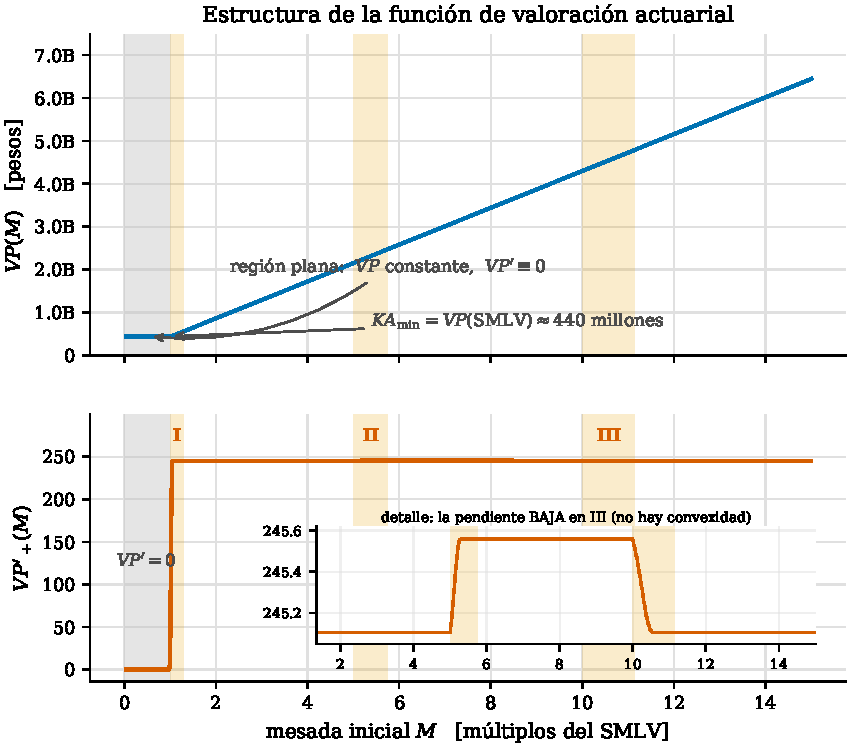
\includegraphics[width=.92\textwidth]{figuras/fig_estructura_vp}
\caption[Estructura de la función de valoración]{Estructura de $\VP$ y de su
derivada lateral derecha. Arriba: la función, con la región plana sombreada en
gris y los tres racimos de quiebres en naranja. Abajo: la derivada, que salta de
$0$ al valor de régimen en el racimo~I. El recuadro interior amplía la variación
fina de la pendiente y revela el hecho decisivo: en el racimo~III la pendiente
\emph{decrece}, lo que prueba que $\VP$ no es convexa
(\cref{thm:no-convexidad}).}
\label{fig:estructura}
\end{figure}

\begin{figure}[H]
\centering
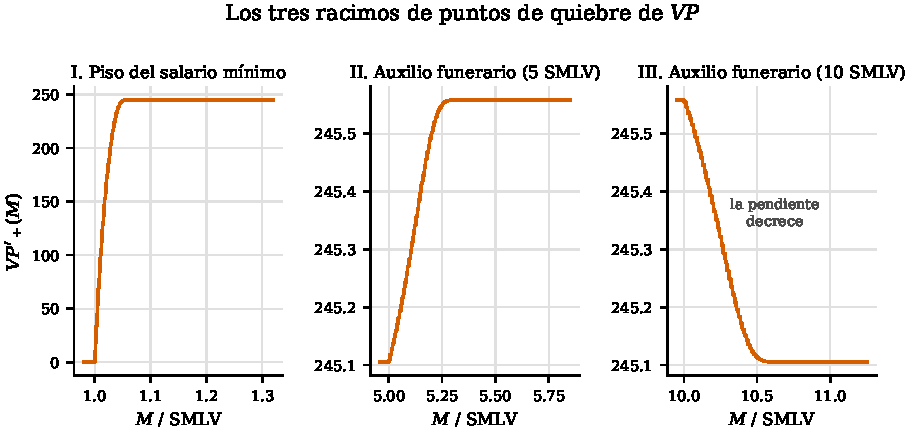
\includegraphics[width=\textwidth]{figuras/fig_zoom_quiebres}
\caption[Los tres racimos de quiebres]{Detalle de los tres racimos. En el
racimo~I la pendiente asciende desde $0$; en el II asciende de nuevo, al activarse
el auxilio funerario; en el III \emph{desciende}, al saturarse el tope de diez
salarios mínimos. Cada conjunto contiene a lo sumo $\datoNAniosMax+1$ quiebres candidatos, uno por año de proyección; los pesos nulos pueden eliminar saltos efectivos, con separaciones geométricas de razón $\datoRhoQuiebre$.}
\label{fig:zoom}
\end{figure}

\section{Convexidad: lo que se conserva y lo que se pierde}

\begin{proposition}[El amparo básico es convexo]
\label{prop:convexidad-rab}
$\VP_{\mathrm{ren}}$ es convexa en $[0,\infty)$.
\end{proposition}
\begin{proof}
Cada $M\mapsto\max\{a_tM,b_t\}$ es el máximo puntual de dos funciones afines,
luego convexo por el \cref{lem:preserva-convexidad}(a). La combinación cónica con
pesos $w_t\ge0$ preserva la convexidad por (b).
\end{proof}

\begin{theorem}[Pérdida de convexidad]
\label{thm:no-convexidad}
Si existe algún $t$ con $c_t>0$ --- es decir, si el contrato cubre auxilio
funerario --- entonces $\VP$ \textbf{no} es convexa en $[0,\infty)$. Concretamente,
la derivada lateral derecha satisface
\[
  \VP'_+\bigl(M\bigr) \;>\; \VP'_+\bigl(M'\bigr)
  \qquad\text{para } M\in\bigl(5\rho_{n_{\max}}S_0,\;10S_0\bigr),\;
  M'>10\rho_{n_{\max}}S_0 .
\]
\end{theorem}
\begin{proof}
Por el \cref{thm:subdiferencial} (que se demuestra a continuación y no depende de
este resultado), para $M$ en el intervalo indicado todos los términos del auxilio
funerario están activos, esto es $5b_t<a_tM<10b_t$ para todo $t$, y por tanto
\[
  \VP'_+(M)\;=\;\sum_t w_ta_t \;+\; \sum_t c_ta_t .
\]
Para $M'>10\rho_{n_{\max}}S_0$ se tiene $a_tM'>10b_t$ para todo $t$, de modo que
todos los términos del auxilio están saturados por arriba y su contribución a la
derivada es nula:
\[
  \VP'_+(M')\;=\;\sum_t w_ta_t .
\]
La diferencia es $\sum_t c_ta_t>0$ por hipótesis. Una función convexa tiene
derivada lateral derecha no decreciente\footnote{El resultado es estándar en análisis convexo; véase \citet[Teorema~24.1]{rockafellar1970} o \citet[§3.1]{boyd2004}. Su contrarrecíproco es lo que se usa aquí: exhibir dos puntos donde la derivada lateral derecha decrece basta para refutar la convexidad, sin necesidad de examinar la función en el resto del dominio.} \citep[Teorema 24.1]{rockafellar1970}; como
aquí decrece, $\VP$ no es convexa.
\end{proof}

Numéricamente, para la póliza de referencia la pendiente pasa de
$\datoPendienteAUF$ en la meseta intermedia a $\datoPendienteAfin$ por encima del
racimo~III: un descenso de $\datoSaltoAUF$ unidades. Es una violación pequeña en
magnitud relativa --- del orden de $2\cdot10^{-3}$ --- pero \emph{cualitativa}\footnote{El auxilio funerario representa una fracción muy pequeña del valor del contrato --- del orden del medio por ciento en la póliza de referencia --- de modo que su efecto sobre la pendiente es necesariamente pequeño. Lo que no es pequeño es su efecto sobre las propiedades cualitativas de la función.}: basta
para invalidar todo argumento que invoque convexidad\footnote{Conviene resistir la tentación de considerar despreciable una violación de dos milésimas. La convexidad es una propiedad cualitativa: o se tiene o no se tiene. Un argumento que la invoque es válido o inválido, y su conclusión no se vuelve \emph{casi} válida porque la violación sea pequeña. Lo que sí es legítimo decir --- y se dice en la \cref{sec:robustez-empirica} --- es que la consecuencia práctica observada es benigna.}.

\begin{criticism}[Consecuencia para la teoría de Newton]
\label{crit:convexidad}
El argumento clásico de convergencia monótona de Newton --- «si $f$ es convexa,
creciente y $x_0>x^*$, entonces $\{x_k\}$ decrece monótonamente hacia $x^*$» ---
descansa en que la tangente quede por debajo de la gráfica. En el racimo~III eso
falla, y la iteración puede sobrepasar la raíz. En la práctica el efecto es
pequeño en los experimentos, pero la hipótesis de convexidad deja de justificar
la convergencia monótona. Una garantía global se obtiene con la salvaguarda de
encaje y bisección periódica del \cref{alg:newton-salvaguardado}, bajo las
condiciones del \cref{thm:salvaguardado}. Este es
el argumento matemático que respalda la recomendación práctica de este trabajo.
\end{criticism}

\section{El subdiferencial y su interpretación actuarial}

\begin{theorem}[Subdiferencial exacto]
\label{thm:subdiferencial}
Para todo $M>0$, el $B$-subdiferencial de $\VP$ es
$\dB\VP(M)=\{\VP'_-(M),\;\VP'_+(M)\}$ con
\begin{align}
  \VP'_+(M) &= \sum_{t:\,a_tM\ge b_t} w_ta_t
             \;+\; \sum_{t:\,5b_t\le a_tM<10b_t} c_ta_t ,
  \label{eq:subdif-der}\\[2pt]
  \VP'_-(M) &= \sum_{t:\,a_tM> b_t} w_ta_t
             \;+\; \sum_{t:\,5b_t< a_tM\le 10b_t} c_ta_t ,
  \label{eq:subdif-izq}
\end{align}
y el subdiferencial de Clarke es
$\dC\VP(M)=\bigl[\min\{\VP'_-,\VP'_+\},\;\max\{\VP'_-,\VP'_+\}\bigr]$.
Si $M\notin\mathcal{B}$, ambos coinciden y $\VP$ es diferenciable en $M$ con
$\VP'(M)=\VP'_\pm(M)$.
\end{theorem}
\begin{proof}
La derivada lateral de $u\mapsto\max\{a_tu,b_t\}$ por la derecha vale $a_t$ si
$a_tu\ge b_t$ y $0$ si no; por la izquierda vale $a_t$ si $a_tu>b_t$ y $0$ si no.
Análogamente, para $u\mapsto\med(5b_t,a_tu,10b_t)$ la derivada por la derecha vale
$a_t$ si $5b_t\le a_tu<10b_t$ y $0$ en otro caso, y por la izquierda vale $a_t$ si
$5b_t<a_tu\le10b_t$. Las derivadas laterales de una suma finita son la suma de las
derivadas laterales; ponderando por $w_t,c_t$ se obtienen
\cref{eq:subdif-der,eq:subdif-izq}. La identificación con $\dB$ y $\dC$ es el
\cref{lem:subdif-pl}.
\end{proof}

\subsection{Qué significa la derivada}
\label{sec:interpretacion-subdif}

La expresión \cref{eq:subdif-der} no es una fórmula opaca. Sustituyendo los
coeficientes de la \cref{prop:forma-canonica}, en la región donde todos los
términos de renta están activos y ninguno del auxilio lo está,
\begin{equation}
\label{eq:derivada-anualidad}
  \VP'(M)\;=\;\frac{1+\gamma}{1-g}\sum_{t=1}^{N}
     \tau_t\,\nu_t\,\kappa_t\,\CONAB(t{+}1)\,v_{t+1}
  \;=\;\frac{1+\gamma}{1-g}\;\ddot a^{(\tau)}_{Y},
\end{equation}
donde $\ddot a^{(\tau)}_{Y}$ es exactamente el \textbf{factor de renta actuarial}
del grupo $Y$: el valor presente de una renta unitaria indexada, pagada
$\kappa_t$ veces por año mientras subsista el derecho.

\begin{aporte}
\textbf{Interpretación.} La derivada de la función de valoración respecto de la
mesada inicial \emph{es} el factor de renta del contrato, recargado por gastos y
cambio de grupo. En consecuencia:
\begin{itemize}[nosep,leftmargin=*]
  \item El paso de Newton $-f(M)/\VP'(M)$ tiene lectura financiera directa: es el
        exceso o defecto de capital dividido por el costo de un peso de mesada
        adicional. Es exactamente el ajuste que un actuario haría a mano.
  \item El subgradiente nunca se anula por encima del salario mínimo, porque es
        una suma de factores de renta estrictamente positivos. Esta es la
        $BD$-regularidad del \cref{thm:bd-regularidad}.
  \item Los dos elementos de $\dB\VP$ en un quiebre corresponden a incluir o
        excluir del factor de renta los periodos en que la mesada está exactamente
        sobre el piso legal.
\end{itemize}
\end{aporte}

Para la póliza de referencia, $\VP'=\datoPendienteAfin$: cada peso adicional de
mesada mensual cuesta $\datoPendienteAfin$ pesos de capital. Recíprocamente, cada
millón de pesos adicional de capital compra $\datoCondicionamientoInverso$ pesos
más de mesada mensual.

\section{Existencia, unicidad y condicionamiento}

\begin{theorem}[Existencia y unicidad en el dominio admisible]
\label{thm:existencia}
En $[S_0,\infty)$ existe una solución única si y solo si
$\KA\ge\KA_{\min}=\VP(S_0)$. En la igualdad es $M^*=S_0$;
para capital estrictamente superior se tiene $M^*>S_0$.
\end{theorem}
\begin{proof}
La función es continua y estrictamente creciente en $[S_0,\infty)$.
Para $M>\rho_{n_{\max}}S_0$, la contribución de renta tiene pendiente
$\sum_t w_ta_t>0$, mientras que el auxilio es no decreciente.
Por tanto $\VP(M)\to\infty$ y su imagen en ese dominio es
$[\VP(S_0),\infty)$. La continuidad da existencia y la monotonía
estricta da unicidad.
\end{proof}

\begin{remark}[Dominio y condición de capital]
La igualdad $\VP(0)=\VP(S_0)$ hace numéricamente equivalentes las
condiciones $\VP(0)<\KA$ y $\VP(S_0)<\KA$. La región plana impide
utilizar monotonía estricta en todo $[0,\infty)$, pero no altera esa
desigualdad. La multiplicidad en la igualdad corresponde al dominio
ampliado; en el dominio admisible la mesada mínima es única.
\end{remark}

\begin{theorem}[Estabilidad de Lipschitz y condicionamiento]
\label{thm:condicionamiento}
Sea $m=\inf\{\,V : V\in\dB\VP(M),\ M\ge \rho_{n_{\max}}S_0\,\}>0$. Para capitales
$\KA_1,\KA_2>\KA_{\min}$ con soluciones
$M_1^*,M_2^*\ge\rho_{n_{\max}}S_0$,
\[
  \bigl|M_1^*-M_2^*\bigr|\;\le\;\frac{1}{m}\,\bigl|\KA_1-\KA_2\bigr| .
\]
Si $M^*$ está en el interior de un tramo afín, el número de condición
relativo del problema es
\[
  \kappa_{\mathrm{rel}}
  \;=\;\frac{\KA}{M^*}\cdot\left|\frac{dM^*}{d\KA}\right|
  \;=\;\frac{\VP(M^*)}{M^*\,\VP'(M^*)} .
\]
\end{theorem}
\begin{proof}
Por el teorema del valor medio para funciones Lipschitz\footnote{Véase \citet[Teorema~2.3.7]{clarke1983}. El enunciado sustituye la derivada del teorema del valor medio clásico por un elemento del subdiferencial de Clarke, y es precisamente la herramienta que permite hacer análisis de estabilidad sobre funciones no diferenciables.}
\citep[Teorema 2.3.7]{clarke1983}, $\KA_2-\KA_1=\VP(M_2^*)-\VP(M_1^*)=V(M_2^*-M_1^*)$
para algún $V\in\dC\VP$ en el segmento, y $V\ge m$. La expresión del número de
condición es la definición usual aplicada a $M^*=\VP^{-1}(\KA)$, cuya derivada es
$1/\VP'(M^*)$ por el teorema de la función inversa, válido porque $\VP$ es afín en
un entorno.
\end{proof}

Para la póliza de referencia, $\kappa_{\mathrm{rel}}=\datoCondRelativa$. Es decir:
\emph{el problema está esencialmente perfectamente condicionado}. Un error
relativo en el capital se traslada casi exactamente, sin amplificación, a un error
relativo en la mesada. Este buen condicionamiento facilita resolver el problema,
pero no garantiza por sí solo que todo método alcance precisión de máquina:
también intervienen su convergencia, las tolerancias y el redondeo. La comparación
de métodos debe contrastar la exactitud alcanzada con el costo de obtenerla.

\section{Semisuavidad y regularidad}

\begin{theorem}[Semisuavidad fuerte]
\label{thm:semisuavidad}
$f=\VP-\KA$ es fuertemente semisuave en todo punto de $[0,\infty)$. Más aún, para
$M\notin\mathcal{B}$ y $|d|$ menor que la distancia de $M$ a $\mathcal{B}$, el
residuo semisuave es \emph{exactamente cero}.
\end{theorem}
\begin{proof}
Es el \cref{lem:pl-semisuave} aplicado a $f$, que es lineal a trozos por la
\cref{prop:pl} con conjunto finito de quiebres $\mathcal{B}$ (\cref{thm:quiebres}).
\end{proof}

\begin{theorem}[$BD$-regularidad]
\label{thm:bd-regularidad}
Sea $M^*>S_0$ una solución. Todo $V\in\dB f(M^*)$ satisface
$V\ge w_1a_1>0$; por tanto $f$ es $BD$-regular en $M^*$.
Si además $M^*>\rho_{n_{\max}}S_0$, se obtiene la cota más fuerte
$V\ge\sum_t w_ta_t>0$.
\end{theorem}
\begin{proof}
Para $M^*>S_0$, el primer término está activo con desigualdad estricta en ambas derivadas, lo que da la primera cota. Para la segunda, ambas derivadas contienen el sumando
$\sum_{t:\,a_tM^*\ge b_t}w_ta_t$ (respectivamente con desigualdad estricta). Como
$M^*>\rho_{n_{\max}}S_0=\max_n b_t/a_t$, todos los índices $t$ están activos con
desigualdad estricta, luego ambas derivadas laterales valen al menos
$\sum_tw_ta_t$. Esta cantidad es positiva porque $w_1>0$ y $a_1=1$.
\end{proof}

\begin{corollary}
\label{cor:qi-sun-aplica}
Para $M^*>S_0$ se cumplen las hipótesis del \cref{thm:qi-sun}; el error
del método de Newton semisuave satisface localmente una cota cuadrática.
Además, como hay un número finito de quiebres, un arranque suficientemente
próximo selecciona un tramo cuya clausura contiene la raíz. El apartado (i)
del \cref{thm:terminacion-finita} da entonces terminación en un paso en
aritmética exacta. Esta terminación local no se interpreta como un orden
asintótico exacto con constante positiva.
\end{corollary}

\begin{remark}[El caso $M^*$ dentro del racimo~I]
Si la solución cae \emph{dentro} del racimo~I --- lo que ocurre cuando el capital
apenas supera el mínimo ---, la $BD$-regularidad sigue valiendo pero con una cota
$m$ mucho menor, pues solo una fracción de los periodos está activa. Es el caso
numéricamente más exigente y el que se aísla en el escenario \texttt{R2} de los
experimentos.
\end{remark}

\section{Un detalle de implementación con consecuencias analíticas}

\begin{proposition}[La distinción de casos es inocua en valor, no en derivada]
\label{prop:continuidad-rama}
Sea $\widetilde{\VP}$ la función definida como $\VP$ salvo que en $M=S_0$ se usa
$\phi_t$ en lugar de $\tau_t$ como factor de crecimiento de la mesada (la
distinción de casos de la \cref{rem:rama-smlv}). Entonces
$\widetilde{\VP}=\VP$ en todo $[0,\infty)$, pero la derivada lateral derecha
calculada con la fórmula \cref{eq:subdif-der} evaluada sobre la rama $\phi$ en
$M=S_0$ difiere de $\VP'_+(S_0)$.
\end{proposition}
\begin{proof}
En $M=S_0$, la rama $\phi$ da $\max\{S_0\phi_t,S_0\phi_t\}=S_0\phi_t=b_t$, y la
rama $\tau$ da $\max\{S_0\tau_t,S_0\phi_t\}=b_t$ porque $\phi_t\ge\tau_t$. Los
valores coinciden, luego $\widetilde{\VP}(S_0)=\VP(S_0)$; fuera de $M=S_0$ las
definiciones son idénticas. Para la derivada, la fórmula \cref{eq:subdif-der}
aplicada con $a_t=\phi_t$ activa \emph{todos} los índices, pues
$S_0\phi_t\ge b_t=S_0\phi_t$ con igualdad, y devuelve $\sum_tw_t\phi_t$; en cambio
la derivada lateral derecha verdadera se calcula sobre la rama $\tau$ y solo
activa los índices con $S_0\tau_t\ge S_0\phi_t$, es decir únicamente $n(t)=0$.
\end{proof}

Numéricamente, la fórmula ingenua devuelve $249{,}06$ en $M=S_0$ frente al valor
correcto $7{,}23$: un factor de $34$\footnote{El valor correcto de la derivada lateral derecha en $M=S_0$ es $7{,}23$, y corresponde a los pocos periodos del año calendario de la valoración en los que el piso aún no se ha separado del nominal. La fórmula evaluada sobre la rama equivocada devuelve $249{,}06$, que es la pendiente que tendría la función si todos los periodos estuviesen activos.}. Un método de Newton que arranque exactamente
en el salario mínimo daría, con la fórmula ingenua, un paso $34$ veces menor del
debido. La implementación de este trabajo corrige el punto seleccionando la rama
$\tau$ para el cálculo de la derivada (recomendación~R2 de la
\cref{sec:hallazgos-codigo}).

\section{Verificación numérica de la estructura}

Los resultados anteriores se contrastaron numéricamente sobre la póliza de
referencia. El \cref{tab:verificacion-estructura} resume esos contrastes, que
ilustran las demostraciones sin sustituirlas.

\begin{table}[H]
\centering
\caption[Verificación numérica de la estructura]{Verificación numérica de los
resultados estructurales sobre la póliza de referencia (hombre de 65 años con
cónyuge de 61, capital \$\,\datoCapitalEjemplo).}
\label{tab:verificacion-estructura}
\small
\begin{tabular}{@{}p{5.6cm}p{4.2cm}p{4.4cm}@{}}
\toprule
\textbf{Resultado} & \textbf{Predicción} & \textbf{Verificación} \\
\midrule
\cref{thm:region-plana}: región plana &
$\VP$ constante en $[0,S_0]$ &
$\VP$ idéntica a $12$ cifras en $M/S_0\in\{0{,}01;\dots;1\}$ \\
\cref{cor:capital-minimo}: capital mínimo &
$\KA_{\min}=\VP(S_0)$ &
$\datoKAmin$ pesos \\
\cref{thm:quiebres}: tres racimos &
$[1;\datoAnchoRacimo]$, $[5;5\cdot\datoAnchoRacimo]$, $[10;10\cdot\datoAnchoRacimo]$ en unidades de $S_0$ &
saltos de $\VP'$ detectados solo en esos tres intervalos
(\cref{fig:zoom}) \\
\cref{cor:region-afin}: región afín &
$\VP(M+d)=\VP(M)+\VP'\!\cdot d$ exacto &
error relativo del orden de $10^{-16}$ para $M\in\{3;6;30\}$ millones \\
\cref{thm:no-convexidad}: no convexidad &
$\VP'$ decrece tras el racimo~III &
$\datoPendienteAUF\to\datoPendienteAfin$ \\
\cref{thm:subdiferencial}: subdiferencial &
coincide con la diferencia central &
coincidencia a $10$ cifras fuera de $\mathcal{B}$ \\
\cref{thm:condicionamiento}: condicionamiento &
$\kappa_{\mathrm{rel}}\approx1$ &
$\datoCondRelativa$ \\
\bottomrule
\end{tabular}
\end{table}

La \cref{fig:residuo-lineal} ofrece la síntesis visual del capítulo. A escala
natural $\VP$ es indistinguible de una recta; restándole la cuerda que une sus
extremos, la estructura lineal a trozos aparece con toda claridad, y su amplitud
relativa resulta ser del orden de $10^{-3}$. El problema es genuinamente no suave
y, al mismo tiempo, genuinamente benigno: ambas cosas a la vez, y esa combinación
es precisamente lo que explica los resultados del \cref{cap:resultados}.

\begin{figure}[H]
\centering
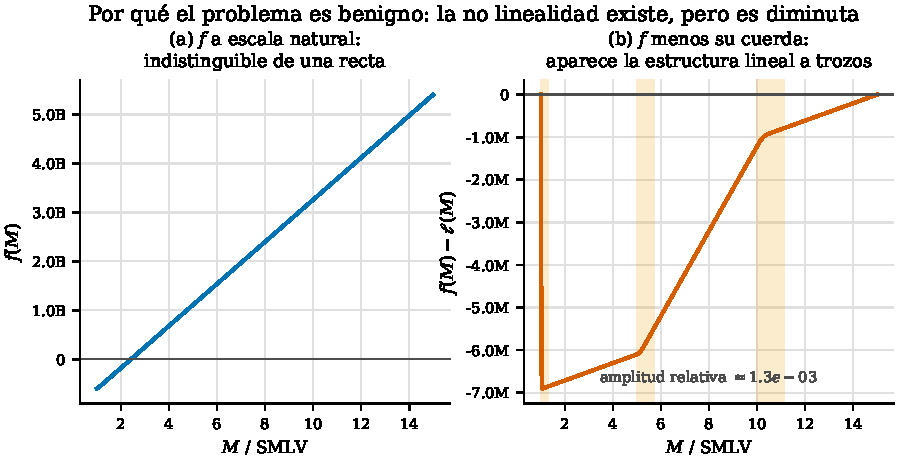
\includegraphics[width=\textwidth]{figuras/fig_residuo_lineal}
\caption[La no linealidad amplificada]{Síntesis del capítulo. A la izquierda, $f$
tal como se ve: una recta. A la derecha, $f$ menos su cuerda, que amplifica la
estructura por un factor de mil y revela los tres racimos de quiebres del
\cref{thm:quiebres} exactamente donde la teoría los predice.}
\label{fig:residuo-lineal}
\end{figure}
